\chapter{Results and Discussion}
\label{ch:results}

\section{Data Availability}

Table~\ref{tab:availability} summarizes field coverage across the 181 O4a events identified (Chapter~\ref{ch:methods}).

\begin{table}[H]
\centering
\caption{Field coverage, O4a observing run (181 events)}
\label{tab:availability}
\begin{tabular}{@{}lrl@{}}
\toprule
Field & Coverage & Notes \\
\midrule
Luminosity distance & 89\% & \textasciitilde half include an explicit uncertainty \\
False alarm rate & 46\% & spans 45 orders of magnitude \\
Source classification & 45\% & mostly BBH in this run \\
Network SNR & 0\% & never the LVK trigger's own value in circular text \\
Orbital inclination & 0\% & not reported in any circular checked \\
Reference chirp mass & 0\% & the bin sentence only appears in later-run circulars \\
\bottomrule
\end{tabular}
\end{table}

\subsection{O4a vs. the Full Archive}

Table~\ref{tab:availability} restricts to O4a as a case study. Repeating the same check across every event in the archive (all observing runs, 505 events) shows coverage is meaningfully \emph{better} once later runs are included: distance 83.6\%, FAR 62.8\%, classification 62.0\%, reference chirp mass 10.1\% (51 events -- the same population behind the validation set in Section~\ref{sec:validation-set}). FAR and classification both improve by roughly 17 percentage points over the O4a-only figures. The likely explanation is that \gls{lvk}'s circular-writing template became more complete and standardized over time, so later-run circulars report more fields consistently than O4a-era ones did -- a small additional finding in its own right: data quality here is improving as the observing program matures, not staying flat.

\subsection{Full Breakdown: Run, Source Class, and Circular Type}
\label{sec:availability-breakdown}

Breaking the same 505-event coverage figures down further, by observing run, by source class, and by circular type, gives a sharper picture than the aggregate numbers above (produced by \texttt{legs/leg1\_estimation/analysis/availability\_analysis.py}; O1/O2 predate the \texttt{S}-prefixed superevent ID scheme this pipeline relies on and are out of scope).

\begin{table}[H]
\centering
\caption{Coverage by observing run}
\label{tab:availability-by-run}
\begin{tabular}{@{}lrrrrr@{}}
\toprule
Run & n & Distance & FAR & Classification & Chirp mass \\
\midrule
O3a & 54 & 72.2\% & 61.1\% & 63.0\% & 0.0\% \\
O3b & 42 & 76.2\% & 54.8\% & 50.0\% & 0.0\% \\
O4a & 181 & 89.0\% & 45.9\% & 44.8\% & 0.0\% \\
O4b & 122 & 90.2\% & 86.1\% & 86.1\% & 0.0\% \\
O4c & 87 & 82.8\% & 78.2\% & 77.0\% & 58.6\% \\
\bottomrule
\end{tabular}
\end{table}

The reference chirp-mass bin sentence is not merely rare before O4c -- it is \textbf{completely absent from every run before it} (0/400 across O3a--O4b) and present in the majority of O4c events (51/87). This sharpens the earlier ``10.1\% overall'' figure into a stronger finding: the circular-only validation set (Section~\ref{sec:validation-set}) is drawn from a single recent observing run by construction, not by coincidence of which events happened to report the field.

\begin{table}[H]
\centering
\caption{Coverage by source class (among 313 classified events)}
\label{tab:availability-by-class}
\begin{tabular}{@{}lrrrr@{}}
\toprule
Class & n & Distance & FAR & Chirp mass \\
\midrule
BBH & 285 & 100.0\% & 99.6\% & 16.8\% \\
NSBH & 11 & 100.0\% & 100.0\% & 0.0\% \\
BNS & 7 & 100.0\% & 100.0\% & 0.0\% \\
Terrestrial & 10 & 90.0\% & 100.0\% & 20.0\% \\
\bottomrule
\end{tabular}
\end{table}

BBH accounts for 285/313 (91\%) of classified events -- the direct, quantified explanation for why every validation set built in this project has been overwhelmingly BBH (Sections~\ref{sec:catalog-validation} and \ref{sec:estimator-comparison}): it reflects the real composition of the archive, not a sampling artifact of this pipeline.

\begin{table}[H]
\centering
\caption{Coverage by circular type (per-circular)}
\label{tab:availability-by-type}
\begin{tabular}{@{}lrrrrr@{}}
\toprule
Type & n & Distance & FAR & Classification & Chirp mass \\
\midrule
Identification & 329 & 94.2\% & 97.9\% & 93.3\% & 15.2\% \\
Update & 361 & 90.0\% & 2.2\% & 8.6\% & 0.8\% \\
Retraction & 58 & 0.0\% & 0.0\% & 0.0\% & 0.0\% \\
External follow-up & 80 & 23.8\% & 3.8\% & 2.5\% & 0.0\% \\
Other LVK & 2{,}796 & 18.6\% & 0.3\% & 0.1\% & 0.0\% \\
\bottomrule
\end{tabular}
\end{table}

FAR, classification, and chirp mass are almost entirely carried by the single initial identification circular; update circulars overwhelmingly revise distance/sky-location and rarely restate the others. This validates a modeling choice already built into the pipeline -- taking the highest-confidence value per field across all circulars for an event is, for FAR/classification/mass, functionally equivalent to reading the identification circular alone, since almost nothing else supplies these fields.

Typical uncertainty when reported: 316/422 (74.9\%) of distance-bearing events include an explicit $\pm$ bound, with median relative half-width 29.2\%; all 51 chirp-mass reference values are bin midpoints with median relative half-bin-width 33.3\% -- a genuinely wide bin, useful context for interpreting the error percentages in Sections~\ref{sec:catalog-validation}--\ref{sec:estimator-comparison}, since an estimate landing within roughly a third of the true value is the same order as the uncertainty already built into the reference value itself. FAR and classification are reported as point values/probabilities with no uncertainty given in circular text, so are not applicable here rather than assigned a fabricated number.

\subsection{Direct vs. Approximated Quantities}
\label{sec:direct-vs-approximated}

Synthesizing the availability findings above against what each estimator actually needs:

\begin{table}[H]
\centering
\caption{Direct vs. approximated quantities}
\label{tab:direct-vs-approximated}
\small
\begin{tabular}{@{}p{2.3cm}p{1.6cm}p{2.6cm}p{3.6cm}p{1.4cm}@{}}
\toprule
Parameter & Availability & Required for & Approximation if missing & Risk \\
\midrule
Luminosity distance & Sometimes (83.6\%) & Both estimators & None -- event dropped & Low \\
False alarm rate & Sometimes (62.8\%) & FAR$\to$SNR proxy only & None -- proxy unavailable & Low--moderate \\
Source classification & Sometimes (62.0\%) & Class baseline, combined model & Falls back to distance-only & Low (Section~\ref{sec:catalog-validation}: adds nothing beyond distance) \\
Network SNR & Essentially never (0\%) & Physics estimator (dominant input) & Fixed $\rho=15$; FAR proxy; real value via catalog crosswalk & \textbf{High} \\
Orbital inclination & Never (0\%) & Physics estimator's $F(\iota)$ & Fixed $\cos\iota = 0.5$ & Moderate, bounded \\
Reference chirp mass (bin) & Sometimes, run-dependent (10.1\% overall, 0\% pre-O4c) & Validation target, not an input & GWTC catalog cross-match (already adopted) & Low once catalog-matched \\
\bottomrule
\end{tabular}
\end{table}

Network SNR stands out as the one parameter this table flags \textbf{High} risk: it is the single largest source of physics-estimator error found in this project, confirmed directly in Section~\ref{sec:catalog-validation} (supplying the real value alone cuts median error from 46.6\% to 31.5\%, with nothing else about the formula changed).

\subsection{Additional Discoveries}

Two findings noticed along the way, beyond the original plan, are worth naming explicitly rather than left implicit: field coverage improving substantially between O4a and O4b/O4c (Section~\ref{sec:availability-breakdown}) reflects \gls{lvk}'s circular-writing template maturing over time, not later events being intrinsically better documented; and sky-localization area (``90\% credible region is $X$~deg$^2$'') appears in \textbf{299/505 events (59.2\%)} -- coverage comparable to \gls{far} and classification, and not currently extracted by this pipeline. It is a plausible secondary parameter for future work (Chapter~\ref{ch:conclusion}), both as a candidate weak proxy for detector-network geometry and as a directly useful retrievable field for the GW Pathfinder leg.

\section{Validation Against the Real GWTC Catalog}
\label{sec:catalog-validation}

The validation set used below (Section~\ref{sec:estimator-comparison}) is limited to what circulars self-report: 49 events, almost entirely \gls{bbh}, and critically, no event with a real network \gls{snr} -- that quantity is structurally absent from circular text (Chapter~\ref{ch:methods}). The public \gls{gwtc} catalog, via the \gls{gwosc} API, removes that limitation: it publishes real, measured chirp mass and real network \gls{snr} for every confirmed event.

\gls{gwtc} event names (e.g. \texttt{GW230627\_015337}) differ from circular superevent IDs (e.g. \texttt{S230627c}), but \gls{gwosc}'s per-event \texttt{gracedb\_id} field gives the exact circular ID directly for any event from 2019 onward -- confirmed directly: \texttt{GW230627\_015337}'s \texttt{gracedb\_id} is \texttt{S230627c}, matching the circular event exactly. Pre-2019 events use an older \texttt{G}-prefixed ID from before the superevent system existed and are out of scope for this cross-match.

Of 380 confirmed post-2019 catalog events, 227 matched to at least one circular in the archive; 153 did not. This gap was checked directly rather than assumed benign: none of the missing IDs appear anywhere in the raw archive text (ruling out a parsing bug), and the missing rate is scattered proportionally across every month from 2019 to 2025 (ruling out a stale archive snapshot, which would only affect the newest months). The actual explanation: median \gls{far} for matched events is $1\times10^{-5}$/yr (highly significant) versus 3/yr for missing events (essentially noise-level). The missing events are low-significance candidates added to the catalog through offline, retrospective analysis after the observing run, which never triggered a real-time public alert circular -- a real, structural ceiling on any circular-based pipeline, independent of this pipeline's own extraction completeness.

Combining circular-extracted distance with catalog-provided real chirp mass and real \gls{snr} gives a 214-event set (4.4$\times$ the circular-only validation set), spanning a genuine mix of source classes. The physics formula was re-tested on this set two ways -- with the real \gls{snr}, and with the same fixed assumed \gls{snr} = 15 used throughout Section~\ref{sec:estimator-comparison} -- using the identical leave-one-out $C$-fitting procedure in both cases, so the \emph{only} difference between the two runs is whether \gls{snr} is real or assumed.

\begin{table}[H]
\centering
\caption{Physics formula, catalog-backed validation (214 events): real vs. assumed SNR}
\label{tab:catalog-results}
\begin{tabular}{@{}lrrrr@{}}
\toprule
SNR source & Median error & Within $\pm25\%$ & MAE & Bias \\
\midrule
Assumed (fixed at 15) & 46.6\% & 58/214 (27\%) & 14.46 M$_\odot$ & +5.79 M$_\odot$ \\
Real (catalog) & 31.5\% & 89/214 (42\%) & 9.18 M$_\odot$ & +2.88 M$_\odot$ \\
\bottomrule
\end{tabular}
\end{table}

Supplying the real \gls{snr} -- with nothing else about the formula, the distance input, or the fitting procedure changed -- cuts the median error by roughly a third and nearly doubles the within-$\pm25\%$ rate. This is a direct, controlled confirmation of the argument built up from first principles and sensitivity analysis earlier in this chapter: \gls{snr} was the dominant error source, not a calibration problem or a flaw in the formula itself. The physics formula is not wrong in the abstract -- it is specifically unusable \emph{from circulars alone}, because circulars cannot supply the one input it depends on most.

Even with real \gls{snr}, 31.5\% median error is still short of the 10--25\% target for most events -- real-world measurement uncertainty, the fixed orientation assumption (never marginalized or measured), and unmodeled detector/pipeline effects absorbed into a single global $C$ all remain. But the gap closed by switching from assumed to real \gls{snr} is the largest single improvement found anywhere in this investigation, larger than calibration alone achieved on the circular-only set.

\subsection{A FAR-to-SNR Proxy, Revisited}

An initial approach to testing whether \gls{far} could substitute for \gls{snr} used a \emph{back-solved} "required $\rho$" -- the SNR value that would make the physics formula match each event's true reference mass -- from just 49 circular-only events, and found only a weak correlation ($r \approx -0.34$): a noisy quantity that conflates the physics formula's own errors with any real \gls{far}-\gls{snr} relationship. Testing directly against 381 real (SNR, FAR) pairs from the catalog instead, fitting $\log(\text{SNR}) = a + b \cdot \log(\text{FAR})$ and validating via leave-one-out, gives $r = -0.70$ and a 10.7\% median SNR-prediction error -- a real, usable relationship, well beyond what the back-solved test suggested.

Accuracy is not uniform across \gls{far}, though (Table~\ref{tab:far-proxy}): the proxy is \emph{least} accurate for the most significant events, likely because many search pipelines cap reported \gls{far} at a floor value (118 of 381 events sit at exactly $1\times10^{-5}$/yr), collapsing a range of true SNRs onto one \gls{far} reading in that regime.

\begin{table}[H]
\centering
\caption{FAR-to-SNR proxy accuracy by FAR range (leave-one-out, 381 events)}
\label{tab:far-proxy}
\begin{tabular}{@{}lrr@{}}
\toprule
FAR range & $n$ & Median SNR-prediction error \\
\midrule
$<10^{-4}$/yr (most significant) & 139 & 19.7\% \\
$10^{-4}$--$10^{-2}$/yr & 46 & 15.6\% \\
$10^{-2}$--1/yr & 73 & 6.7\% \\
$>1$/yr (least significant) & 123 & 5.6\% \\
\bottomrule
\end{tabular}
\end{table}

Applying the proxy downstream -- predicting \gls{snr} from each circular's own extracted \gls{far}, then feeding that into the physics formula with the same leave-one-out $C$-fitting procedure used throughout -- gives a real but modest improvement on the 49-event circular-only set: median error falls from 44.8\% (fixed \gls{snr} = 15) to 39.5\%, within-$\pm25\%$ rises from 13/49 to 16/49. This smaller-than-expected gain is traceable, not mysterious: the 49 circular-only events have a median \gls{far} of $4.1\times10^{-3}$/yr, squarely in the harder 15.6\%-error band above, not the easy 5--6\% band. None of these 49 events are themselves in the catalog yet -- they postdate the latest GWTC release -- so the proxy's accuracy on this exact population cannot be checked directly; the FAR-stratified result is the best available evidence for what to expect.

\subsection{Revisiting the Combined Class+Distance Model}

Section~\ref{sec:estimator-comparison} below reports that extending the distance-only statistical model with source classification was attempted and abandoned earlier in this investigation: the 49-event circular-only set is 48/49 (98\%) \gls{bbh}, with no real class diversity to test against. The 214-event catalog-backed set is different -- 206 \gls{bbh}, 5 \gls{nsbh}, 2 Terrestrial, 1 \gls{bns}. Still thin for \gls{nsbh}/\gls{bns} individually (a single-example \gls{bns} dummy would have zero degrees of freedom and simply memorize that one point), so classification enters as a single binary predictor (\gls{bbh} vs. everything else) rather than per-class dummies -- a real limitation, stated rather than hidden. On the 212 non-Terrestrial events:

\begin{table}[H]
\centering
\caption{Distance vs. class vs. combined, 212-event catalog-backed set (Terrestrial excluded)}
\label{tab:combined-model}
\begin{tabular}{@{}lrrr@{}}
\toprule
Model & Median error & Within $\pm25\%$ & Within $\pm50\%$ \\
\midrule
Distance only & 27.8\% & 98/212 (46\%) & 146/212 (69\%) \\
Class only (BBH vs. not) & 38.5\% & 58/212 (27\%) & 135/212 (64\%) \\
Distance + class (combined) & 28.9\% & 98/212 (46\%) & 149/212 (70\%) \\
\bottomrule
\end{tabular}
\end{table}

This time the answer is clean rather than ambiguous: distance alone is the stronger single predictor, and adding class on top of it does not meaningfully help (28.9\% vs. 27.8\% median -- marginally worse, not better). With real class diversity available, this properly resolves what the 49-event set could not test: class does not add independent signal beyond distance, at least at this sample size and with a binary class split.

A second, unplanned finding sits alongside this: distance-only on the larger, more diverse 212-event set (27.8\% median) is competitive with -- and by this metric, marginally better than -- the physics formula given real catalog \gls{snr} (31.5\%, above). The simplest circular-derivable statistical model matches or exceeds a physically-motivated formula that requires information circulars cannot supply.

\subsection{Run-Specific Calibration}

The M6.2 checklist named this as untested: does fitting the physics formula's calibration constant $C$ separately per observing run, rather than one constant across all runs, reduce error? Now that named run windows exist for every run (Section~\ref{sec:availability-breakdown}) and the 214-event catalog-backed set spans four of them with real \gls{snr}, this is directly testable (\texttt{legs/leg1\_estimation/validate\_run\_stratified\_calibration.py}), leave-one-out at every level.

\begin{table}[H]
\centering
\caption{Global vs. run-specific vs. era-specific calibration}
\label{tab:run-calibration}
\begin{tabular}{@{}lrrr@{}}
\toprule
Calibration & Median error & Within $\pm25\%$ & Within $\pm50\%$ \\
\midrule
One global $C$ (all 214 events) & 31.5\% & 88/214 (41\%) & 171/214 (80\%) \\
Per-run $C$ (O3a/O3b/O4a/O4b) & 26.6\% & 97/214 (45\%) & 175/214 (82\%) \\
Per-era $C$ (O3 vs.\ O4) & 26.6\% & 98/214 (46\%) & 177/214 (83\%) \\
\bottomrule
\end{tabular}
\end{table}

Splitting by run helps, but not uniformly, and the reason is itself informative: the fitted $C$ splits cleanly by era ($C \approx 8.8$--$8.9\times10^{-5}$ for O3a/O3b vs.\ $C \approx 5.86$--$5.90\times10^{-5}$ for O4a/O4b, a genuine $\sim$50\% difference, consistent with real detector-network changes between the two eras) -- but per-run leave-one-out calibration only pays off for the two larger runs (O4a: 32.0\%$\to$23.9\%, O4b: 33.9\%$\to$27.3\%) and makes the two smaller runs \emph{worse} (O3a: 21.1\%$\to$33.4\%, O3b: 25.5\%$\to$35.3\%), since refitting on only 18--25 events is unstable. Merging to era level (O3 vs.\ O4, $n=43$ and $n=170$) recovers essentially all of the run-level benefit while avoiding that small-sample instability -- the version worth keeping.

\section{Estimator Comparison (Circular-Only Validation)}
\label{sec:estimator-comparison}

Table~\ref{tab:results} reports leave-one-out cross-validation results on the 49-event circular-self-reported validation set (Section~\ref{sec:validation-set}).

\begin{table}[H]
\centering
\caption{Estimator comparison, 49-event validation set, leave-one-out}
\label{tab:results}
\begin{tabular}{@{}lrrr@{}}
\toprule
Estimator & Median error & Within $\pm25\%$ & Correct bin \\
\midrule
Physics, C fixed (literature value) & 115\% & 5/49 (10\%) & 7/49 (14\%) \\
Physics, C properly fit (LOO) & 45\% & 13/49 (27\%) & 20/49 (41\%) \\
Statistical (distance only) & 33\% & 17/49 (35\%) & 25/49 (51\%) \\
Baseline: source-class midpoint & 50\% & 23/49 (47\%) & 23/49 (47\%) \\
Baseline: population average (LOO) & 50\% & 0/49 (0\%) & 23/49 (47\%) \\
\bottomrule
\end{tabular}
\end{table}

Adding \gls{far} or \gls{bbh}-classification probability as additional regression predictors did not improve the statistical model (median error rose to 36--41\%); with only 49 samples, extra predictors overfit rather than add signal, and \gls{bbh} probability has little variance across the sample (mostly 96--99\%).

\subsection{Calibration Findings}

The methodology note's $C = 1\times10^{-4}$ was fit on a single worked example, not against data. Fitting it properly (Section~\ref{sec:calibration}) gives a fitted $C \approx 5.6\times10^{-5}$ -- about 1.8 times smaller than the literature value -- and cuts the physics formula's median error from 115\% to 45\%. The fitted $C$ is stable across folds (5.44 to 5.78 $\times10^{-5}$ across all 49 leave-one-out refits), so instability in $C$ is not the limiting factor.

Even with a properly fit $C$, the physics formula's log-residuals correlate with log-distance at $r = 0.55$ -- a substantial systematic bias. $C$ is a single global constant, but the fixed-\gls{snr} assumption it stands in for is intrinsically distance-dependent in reality (true \gls{snr} falls off with distance; the model holds it fixed). No choice of $C$, however well fit, can absorb a bias that varies systematically with an input the model treats as constant -- clear evidence the physics formula's shortfall is structural, not a calibration problem. Figures~\ref{fig:physics-uncal-dist} and \ref{fig:physics-cal-dist} show this directly: calibration compresses the error scale (roughly 700\% down to 400\% at maximum) but the same rising-with-distance shape persists.

\begin{figure}[H]
\centering
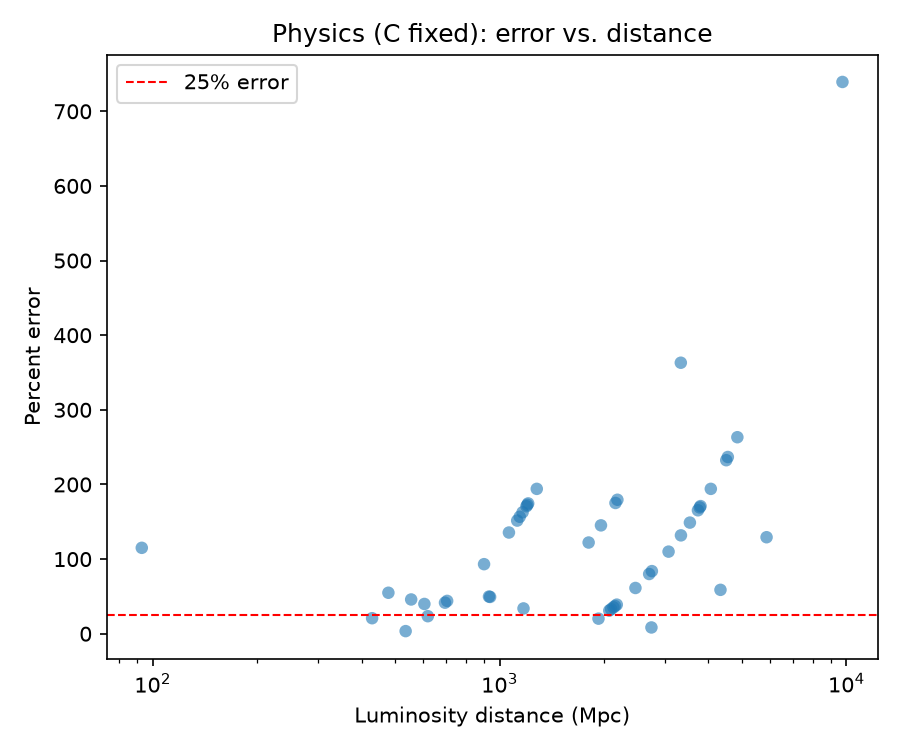
\includegraphics[width=0.75\textwidth]{figures/physics_uncalibrated_vs_distance.png}
\caption{Physics estimator, uncalibrated $C$: percent error vs. luminosity distance. Error rises sharply and consistently with distance.}
\label{fig:physics-uncal-dist}
\end{figure}

\begin{figure}[H]
\centering
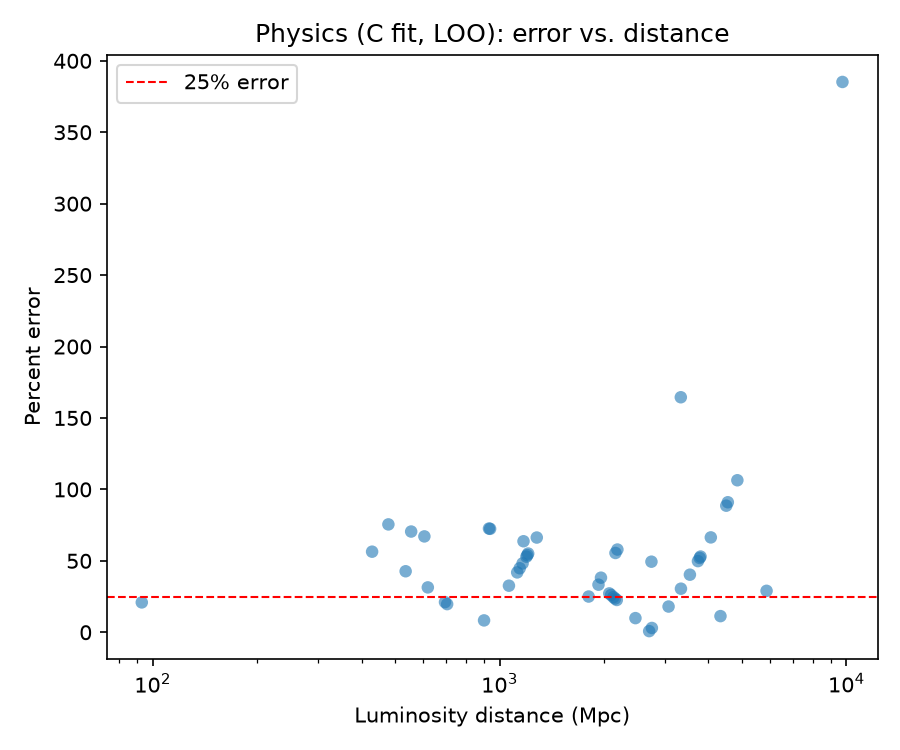
\includegraphics[width=0.75\textwidth]{figures/physics_calibrated_vs_distance.png}
\caption{Physics estimator, $C$ properly fit (leave-one-out): percent error vs. luminosity distance. The same rising trend survives calibration, at a compressed scale.}
\label{fig:physics-cal-dist}
\end{figure}

\subsection{The Trivial Baseline Finding}

A source-class-midpoint baseline -- no distance, no fitting, no per-event information beyond the classification label -- achieves a 47\% within-$\pm25\%$ rate and a 47\% bin-hit rate, both close to (and on the $\pm25\%$ metric, better than) the distance-only statistical model's 35\%/51\%. The initial explanation for this (that distance and source class are correlated, since heavier \gls{bbh} systems are both louder and visible further out) does not hold up: the 49-event validation set is 48/49 (98\%) \gls{bbh}, with only one unclassified event and zero \gls{bns}/\gls{nsbh}. There is essentially no class diversity in this sample to correlate distance against. The baseline's competitiveness more plausibly reflects that guessing near the sample's dominant, modal value is a strong strategy when the sample is this concentrated -- not evidence of a genuine distance-class relationship. The population-average baseline, by contrast, is uniformly poor (0\% within $\pm25\%$), confirming that per-event structure of \emph{some} kind is genuinely needed. Whether class adds signal beyond distance specifically could not be established on this 49-event sample -- but is resolved directly in Section~\ref{sec:catalog-validation} using the catalog-backed set's real class diversity.

\begin{figure}[H]
\centering
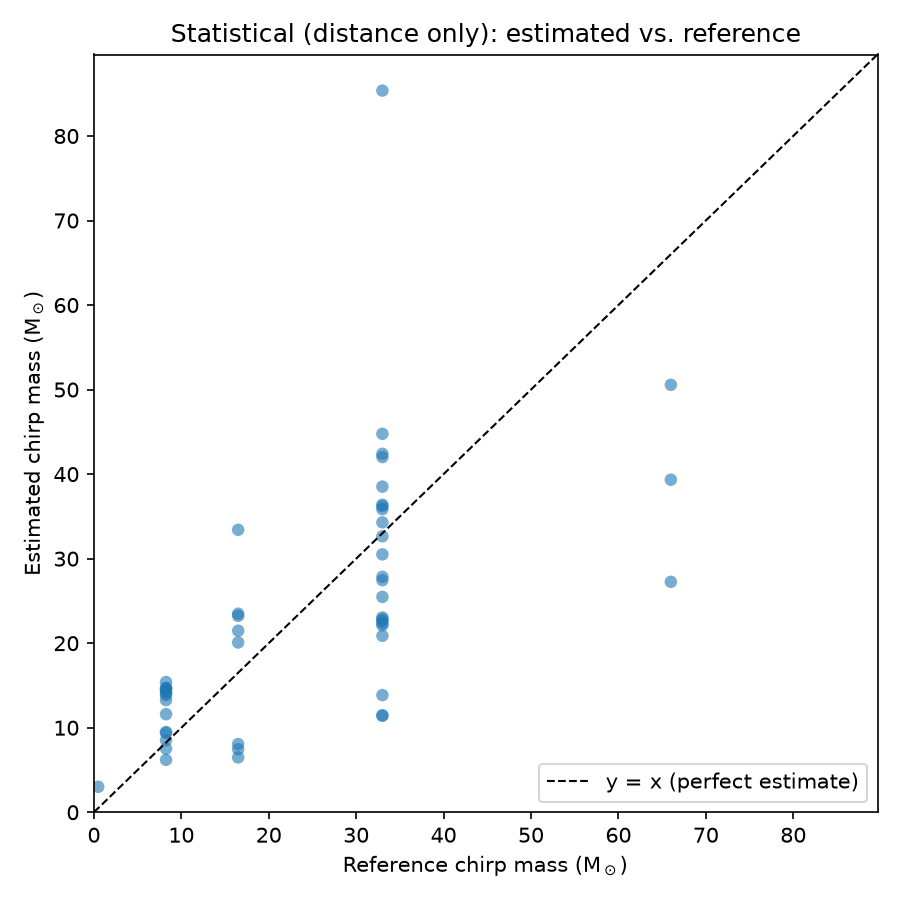
\includegraphics[width=0.75\textwidth]{figures/statistical_scatter.png}
\caption{Statistical estimator: estimated vs. reference chirp mass. The vertical banding reflects the reference values themselves being quantized into LVK's discrete mass bins (midpoints at 8.25, 16.5, 33, 66 M$_\odot$), not continuous measurements.}
\label{fig:statistical-scatter}
\end{figure}

\subsection{Decision-Gate Classification}

Following the project's decision-gate taxonomy (\texttt{validated\_approximation} $\mid$ \texttt{useful\_constraint} $\mid$ \texttt{exploratory\_only} $\mid$ \texttt{unsupported}):

\begin{itemize}
    \item \textbf{Physics (SNR-scaling) estimator, circular-only inputs: \texttt{unsupported}.} Fails even after properly fitting its calibration constant, with a systematic, physically-explained bias that no calibration choice removes -- because the one input it depends on most (\gls{snr}) is structurally absent from circular text. Section~\ref{sec:catalog-validation}'s catalog validation clarifies the scope of this: the formula itself is not unsupported in the abstract (given real \gls{snr}, it more than halves its own error), only as a circular-derived estimator specifically. Era-specific calibration (O3 vs.\ O4) closes a further, smaller slice of that gap (31.5\%$\to$26.6\%, Section~\ref{sec:catalog-validation}), but SNR remains the dominant lever by a wide margin.
    \item \textbf{Statistical (distance-only) estimator: \texttt{useful\_constraint}.} Not a validated per-event measurement, but a real, reproducible signal (best \gls{mae} and bin-hit rate of any method tested) useful for narrowing the plausible mass range. On the small circular-only set, a zero-fitting class-based baseline looked competitive, raising the question of whether distance was an independently powerful signal or just correlated with class; the larger catalog-backed set answers this directly (Section~\ref{sec:catalog-validation}) -- distance alone outperforms class alone and combining the two does not improve on distance alone, so the signal is genuinely distance's, not borrowed from classification.
\end{itemize}

\section{AI-Model Comparison Study}

% TODO: this section is a placeholder pending the fresh comparison batch
% planned for Days 6-7 of the sprint. Initial (~50-event) results using a
% structured Role/Task/Context/Reasoning/Output/Stopping prompting framework
% across five free-tier LLMs (ChatGPT, Gemini, Claude, DeepSeek, Grok) showed
% inconsistent reliability -- some models correctly identified non-BBH events
% and cited catalogs cleanly, others gave partial or unverifiable answers
% from memory alone. Full results and analysis to be added here.

\section{GW Pathfinder Evaluation}

% TODO: pending the minimal prototype build (sprint Days 8-10). This section
% will report the M9.4 test-question evaluation (factual retrieval,
% comparison, filtering, out-of-scope categories) once the prototype exists.
